%# -*- coding: utf-8-unix -*-
% !TEX program = xelatex
% !TEX root = ../thesis.tex
% !TEX encoding = UTF-8 Unicode
%%==================================================
%% chapter02.tex for SJTU Master Thesis
%% based on CASthesis
%% modified by wei.jianwen@gmail.com
%% Encoding: UTF-8
%%==================================================

\chapter{Key nodes selection on two-layers network}
\label{chap5}
In this chapter, it would be investigated that which nodes have the most important influence for keeping or changing their orientation on two-layer networks. There exist many methods to select key nodes, such as pagerank, degree centrality, eigenvector centrality, betweenness centrality and closeness centrality. And, in \parencite{mesgari2015, huang2014}, it has been proved that multiple indicators,that use the rank difference of several node centralities, are useful to identify key nodes and prevent the slow way to identify important nodes. Based on these methods such as single node centrality(single indicator) and combined node centrality(multiple indicator), it would be researched that which method is the most effective and the most influential for selecting key nodes.  

\section{Method for selecting key nodes}
\label{sec:method for finding key nodes}
As the initial condition for selecting key nodes, each layer is made of \textit{BA} network with $512$ nodes, $K=3$, and $1$ external edge. Each simulation takes $100$ steps, and $100$ simulations are considered for average results. To clearly demonstrate the influence of key nodes, the parameters such as $p$ and $v$ would be set to be the opposite consensus state to a layer for identifying key nodes. And then the stubborn nodes that do not change their states are selected by using methods for selecting key nodes and the ratio of stubborn nodes is increased until the state of network is changed into same consensus state with the layer. Under these conditions, the most influential method would be the fastest method to reach the same consensus state with a layer for selecting key nodes. For example, for selecting key nodes on layer A, the parameters would be set to be negative consensus state. Then, as the stubborn nodes on layer A are selected by node centrality or other method and the ratio of the stubborn nodes is increased, the network state would be gradually changed into positive state. Inversely for selecting key nodes on layer B, the parameters would be set to be positive consensus state. Then, as the stubborn nodes on layer B are selected by the method for recognizing key nodes and the ratio of stubborn nodes is increased, the network state would be gradually changed into negative state. Here, we would try to find the fastest and the most influential method.

As the method to select stubborn nodes, we would use two kinds of indicators, single indicator and multiple indicator. As single indicators, node centralities would be applied such as pagerank, degree, eigenvector, closeness and betweenness. As multiple indicators, combined node centralities that consists of several node centralities would be applied.
  
First, here is the way to select key nodes by using a single node centrality.
\begin{enumerate}
	\item All nodes are ranked by 5 node centralities(pagerank, degree, eigenvector, closeness, betweenness).
	\item The nodes are deactivated from high ranked order until the state of network has significant difference, i.e. the stubborn nodes are selected according to high ranked order and the ratio of stubborn nodes is increased. 
	\item The results are compared according to node centralities. When a node centrality makes the state of network reach the fastest to the same consensus with the layer or have the largest change, it would be the most influential method for selecting key nodes.
	\item To clarify which method is the most effective, each single indicator is calculated with summation of all $AS$, that represents `Average States' of network, according to the ratio of stubborn nodes. It is recognized that the larger the $AS$ value is on layer A, the more influential that indicator is, inversely the smaller the $AS$ value is on layer B, the more influential that indicator is.
	
\end{enumerate}
And, we would research the way to recognize important node by using multiple indicators such as combined node centralities(\textit{PR+DE, PR+BE, DE+BE, PR+DE+BE}). Combined node centralities are made up with several selected node centralities. When it is proven that a node centrality is effective for selecting key nodes through the simulations, it would be selected as a factor of combined node centrality. Here, $2$ or $3$ node centralities would be selected such as pagerank, degree and betweenness. 
The way to recognize key nodes by using combined node centrality follows like this steps. 
\begin{enumerate}
	\item All nodes are ranked by each selected node centrality. All nodes has the ranks as the number of selected node centralities.  
	\item Combined node centrality is calculated by the summation of all ranks which a node has. 
	\item All nodes are ranked again by combined node centrality. The smaller the combined node centrality is, the higher a node are ranked.        
	\item The nodes are deactivated from high ranked order until the state of network has significant difference, i.e. the stubborn nodes are selected according to high ranked order and the ratio of stubborn node is increased. 
\end{enumerate}

It has been already proven that single node centrality has good performance to identify key nodes.\parencite{koschutzki2008, francisco2019, bianconi2018}. However, identifying key nodes by multiple indicators is still open problem because there are lots of ways to set up and optimize the weight of each node centrality.\parencite{huang2014}  Here, we simplify the method by setting the weights as equal and simply calculate the summation of ranks. Though our multiple indicators need to be researched further, the multiple indicators would be evaluated and compared with single indicators.\\
 
\section{Key nodes on layer A}
\begin{figure}[!htb]
	\centering
	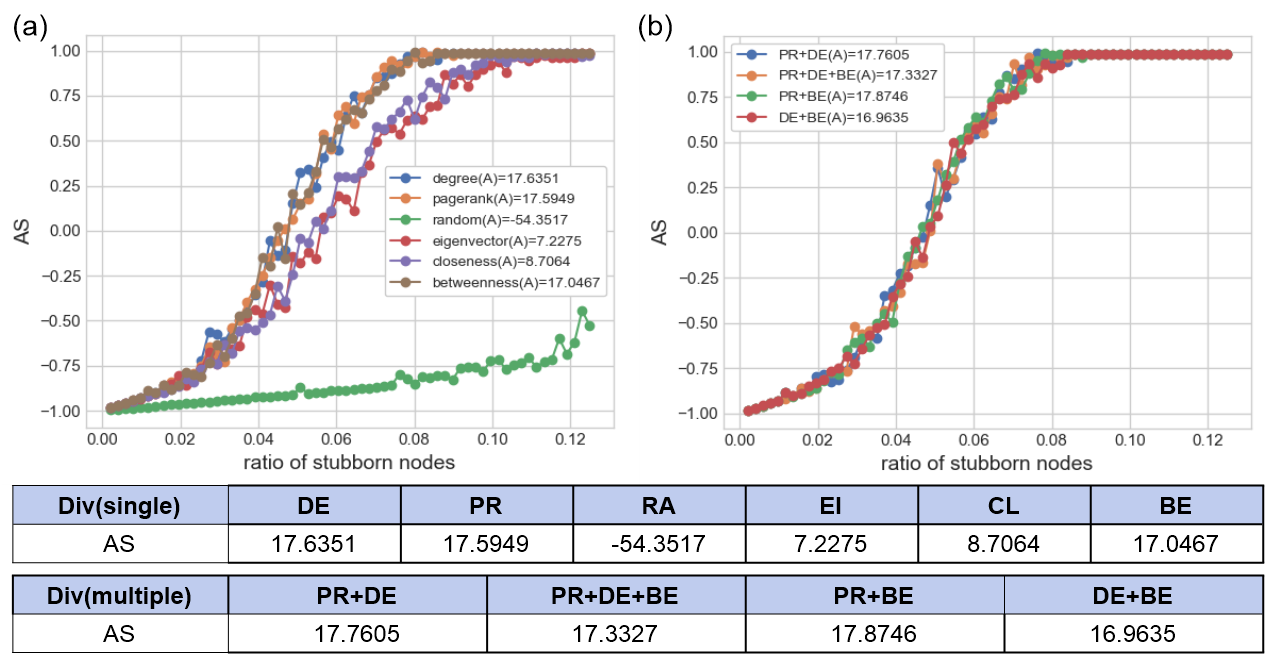
\includegraphics[width=\hsize]{figure/chap5_keynode_A.png}
	\caption{Key nodes on layer A in \textit{BA(3)-BA(3)} network($p=0.2, v=0.4$): (a) Single indicator methods, (b) Multiple indicator methods}
	\label{chap5_keynode_A}
\end{figure}
To select key nodes on layer A, parameters are set to be negative consensus state like $p=0.2, v=0.4$.  As single indicators, 5 node centralities(pagerank, degree, eigenvector, closeness, betweenness) are used, and randomly selected nodes are compared with $5$ node centralities. As multiple indicators, $2$ or $3$ node centralities are combined such as pagerank, degree and betweenness which have the good performance as single indicators. In combined node centralities, we denote pagerank, degree and betweenness as \textit{PR, DE, BE}. And when they are combined, the methods are denoted as \textit{PR+DE, PR+BE, DE+BE, PR+DE+BE} by using \textit{+}. 

Fig.~\ref{chap5_keynode_A} shows the simulation result for recognizing key nodes on layer A. As a single indicator, pagerank has the best performance. The next ranks are degree and betweenness. As a multiple indicator, \textit{PR+BE} has the most effective result. The next is \textit{PR+DE}. These two methods of multiple indicators work better than pagerank. Totally, compared with all methods, the best method is \textit{PR+BE}. It could be found out that some multiple indicators are more effective for selecting key nodes than single indicators. \\

\section{Key nodes on layer B}
\begin{figure}[!htb]
	\centering
	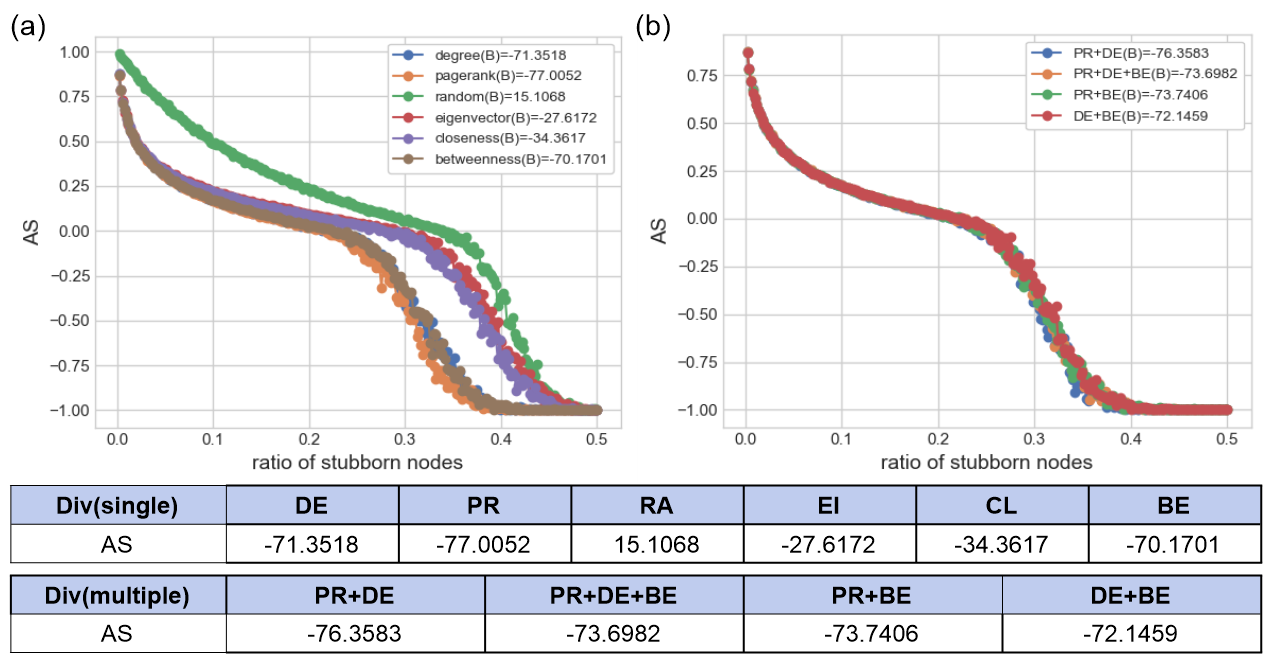
\includegraphics[width=\hsize]{figure/chap5_keynode_B.png}
	\caption{Key nodes on layer B in \textit{BA(3)-BA(3)} network($p=0.3, v=0.5$): (a) Single indicator methods, (b) Multiple indicator methods}
	\label{chap5_keynode_B}
\end{figure}

To select key nodes on layer B, parameters are set to be positive consensus state like $p=0.3, v=0.5$.\\
Fig.~\ref{chap5_keynode_B} shows the simulation result for identifying key nodes on layer B. As a single indicator, the most effective way to recognize important nodes is pagerank centrality. The next ranks are degree and betweenness. As a multiple indicator, \textit{PR+DE} has the best performance. Totally, pagerank is the most effective method for selecting key nodes on layer B. However, all multiple indicators work better than degree centrality, the second rank in single indicators. It could be found out that combined node centralities also have the good performance for selecting key nodes, though they are not the best. \\

\section{Key nodes on two layers with different structures}
In this section, we would try to select the key nodes in the networks with various structures, that are described in chapter.\ref{chap2}. Node centralities and combined node centralities are also used as the methods for selecting key nodes. First, \textit{Hierarchical Model} would be applied to identify important nodes. Second, we would consider the case that each layer has different network type, such as \textit{BA-RR} or \textit{RR-BA} networks. Third, the case would be considered that each layer has different number of internal edges. Layer A could have more internal links or layer B could have more internal links. Both cases would be checked. \\

\subsection{Key nodes in Hierarchical Model}
\begin{figure}[!htb]
	\centering
	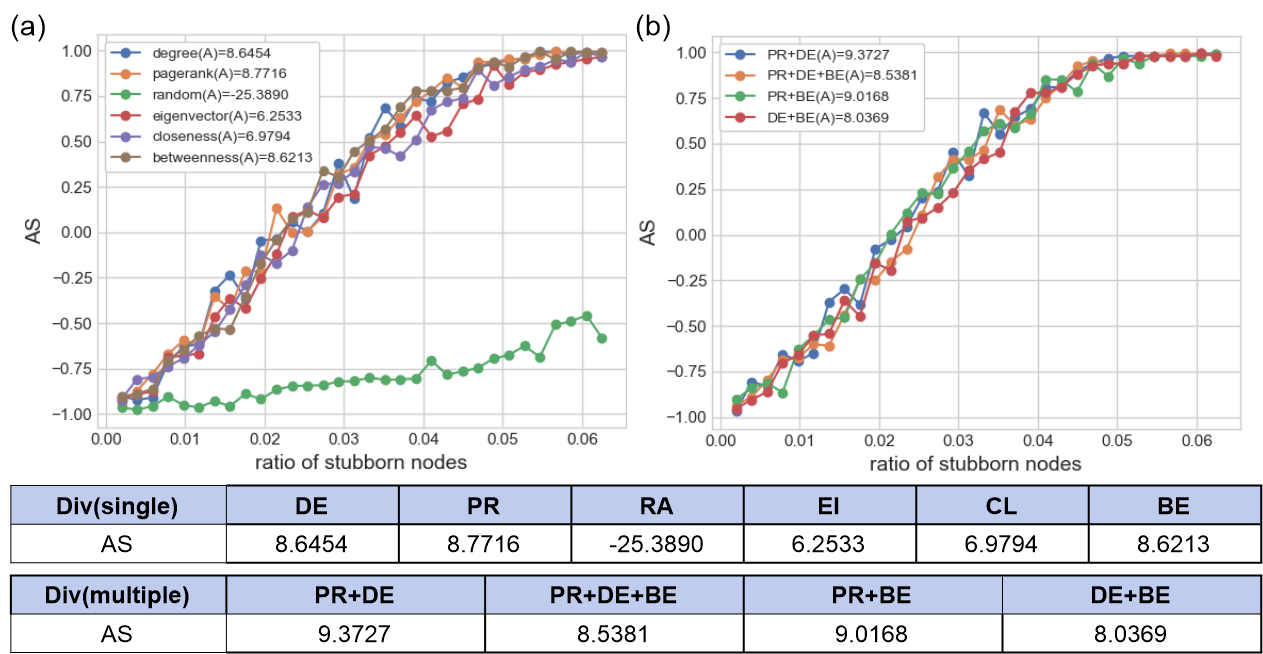
\includegraphics[width=\hsize]{figure/chap5_keynode_HM_A.png}
	\caption{Key nodes on layer A in \textit{Hierarchical Model(8)}($p=0.2, v=0.2$):
		(a) Single indicator methods, (b) Multiple indicator methods}
	\label{chap5_keynode_HM_A}
\end{figure}
\begin{figure}[!htb]
	\centering
	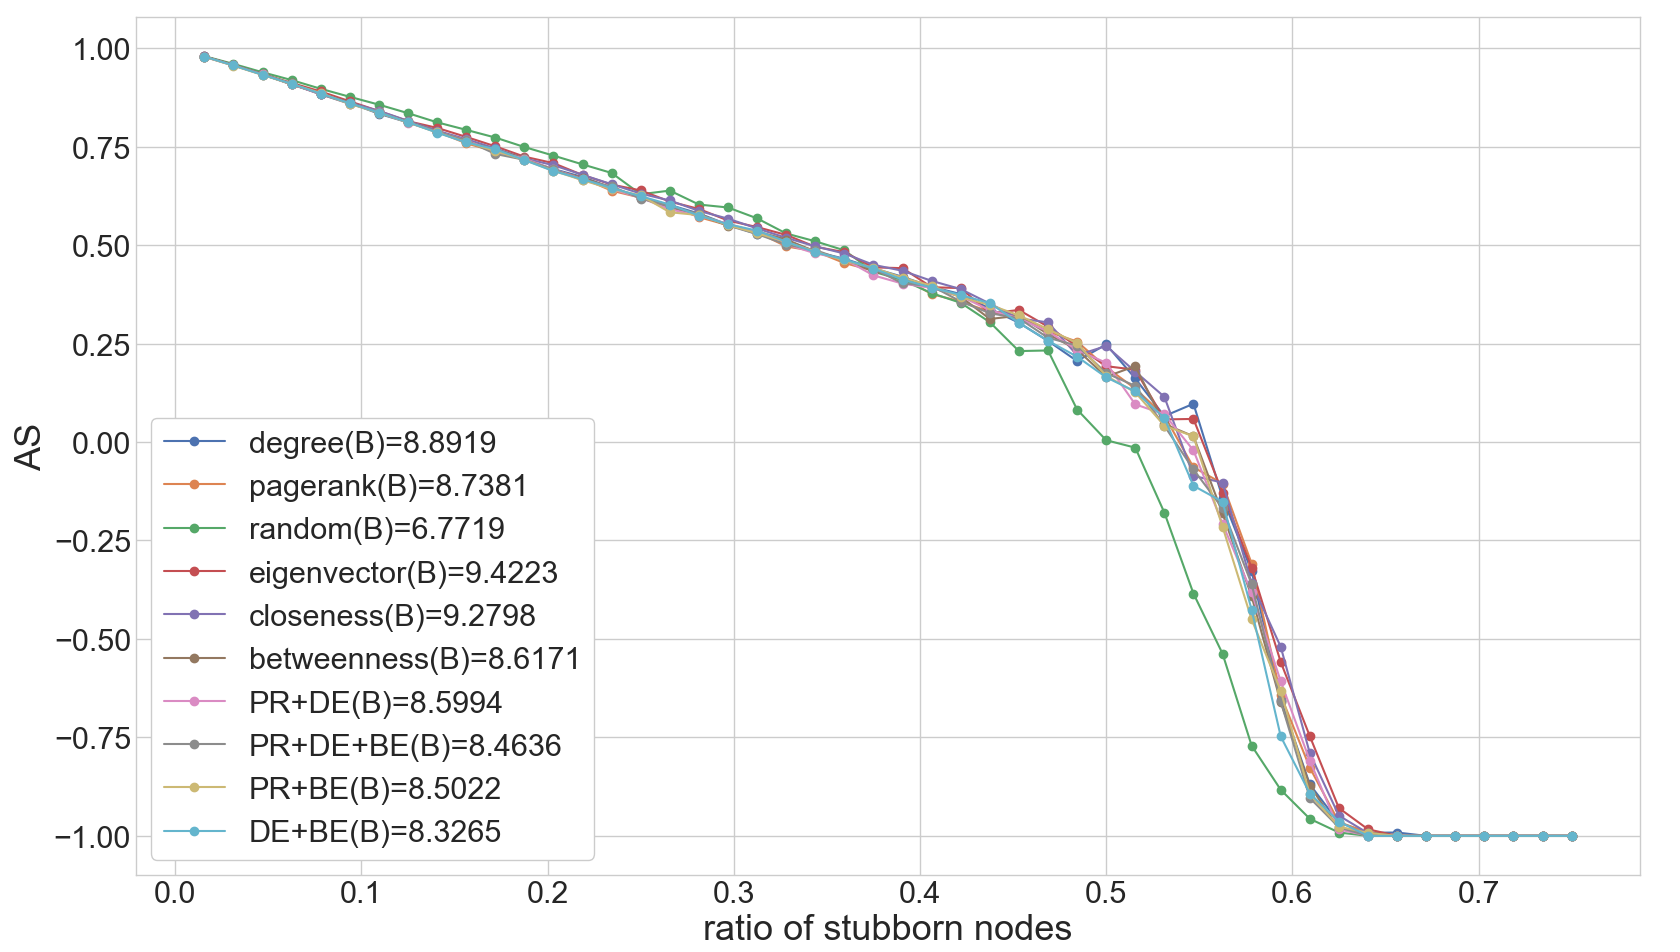
\includegraphics[width=\hsize]{figure/chap5_keynode_HM_B.png}
	\caption{Key nodes on layer B in \textit{Hierarchical Model(8)}($p=0.25, v=0.3$):
		(a) Single indicator methods, (b) Multiple indicator methods}
	\label{chap5_keynode_HM_B}
\end{figure}

Each layer consists of \textit{BA} network with $k=3$. Layer A has $512$ nodes, and layer B has $64$ nodes. We denote these models as \textit{HM(8) with BA(3)}.

Fig.~\ref{chap5_keynode_HM_A} shows the simulation result of key nodes on layer A. Simulations result shows that \textit{PR+DE} is the best method for recognizing key nodes on \textit{HM(8)}. Next ranks are \textit{PR+BE} and pagerank. The curve of changing the network states shown in Fig.~\ref{chap5_keynode_HM_A} is more straight than Fig.~\ref{chap5_keynode_A}. That means the speed of changing network states is faster. 

Fig.~\ref{chap5_keynode_HM_B} shows the simulation result of key nodes on layer B. However, the result is different from other simulation results. The best performance method is random method. That means node centralities do not work on this model. And the curve of changing the network states shown in Fig.~\ref{chap5_keynode_HM_B} is also more straight than Fig.~\ref{chap5_keynode_B}, that means the consensus is easier and the consensus time is shorter. It is found out that \textit{Hierarchical Models} make it hard to recognizing key nodes on layer B and make it easy to have consensus of two layers by stubborn nodes. \\

\subsection{Key nodes on two layers with different network types}
Here, we would consider two types of network, \textit{BA-RR} and \textit{RR-BA}. The number of internal links on each layer would be set up as same or almost same number to exclude the influence of internal links. These models would be compared with \textit{BA-BA} to find out the influence of network types under same conditions, such as $p$, $v$, and $ratio of stubborn nodes$.  

\begin{figure}[!htb]
	\centering
	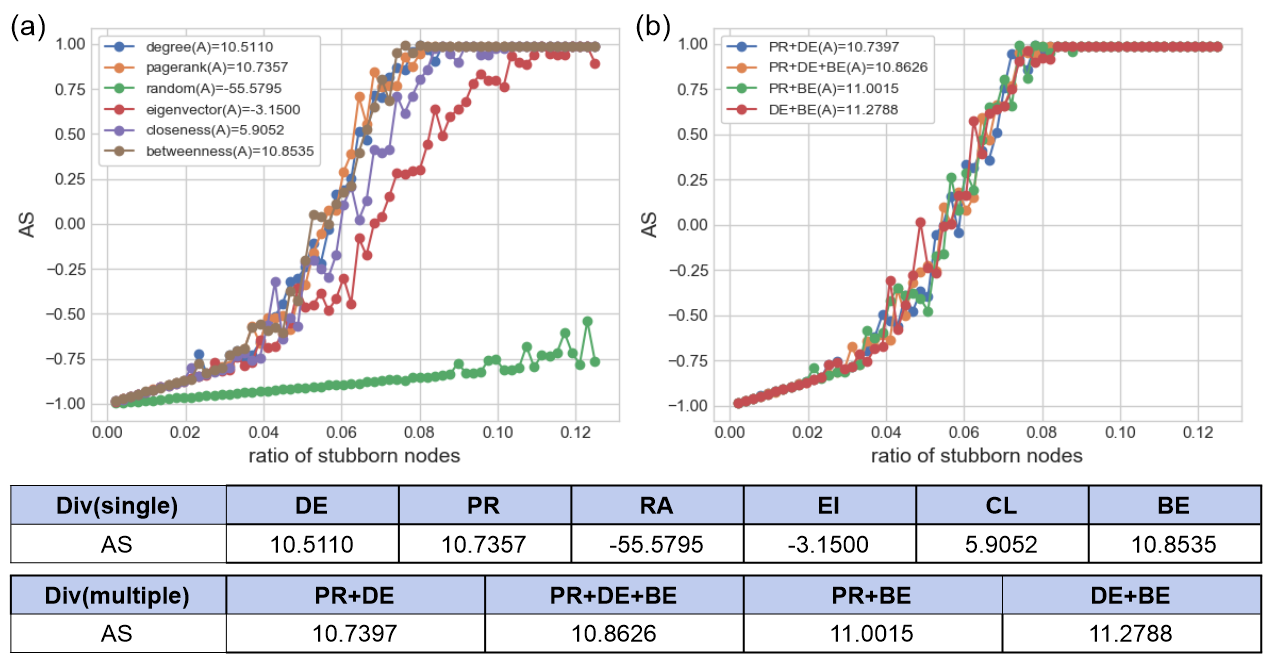
\includegraphics[width=\hsize]{figure/chap5_keynode_BA_RR_A.png}
	\caption{Key nodes on layer A in \textit{BA(3)-RR(6)} network($p=0.2, v=0.4$):
		(a) Single indicator methods, (b) Multiple indicator methods}
	\label{chap5_keynode_BA_RR_A}
\end{figure}
\begin{figure}[!htb]
	\centering
	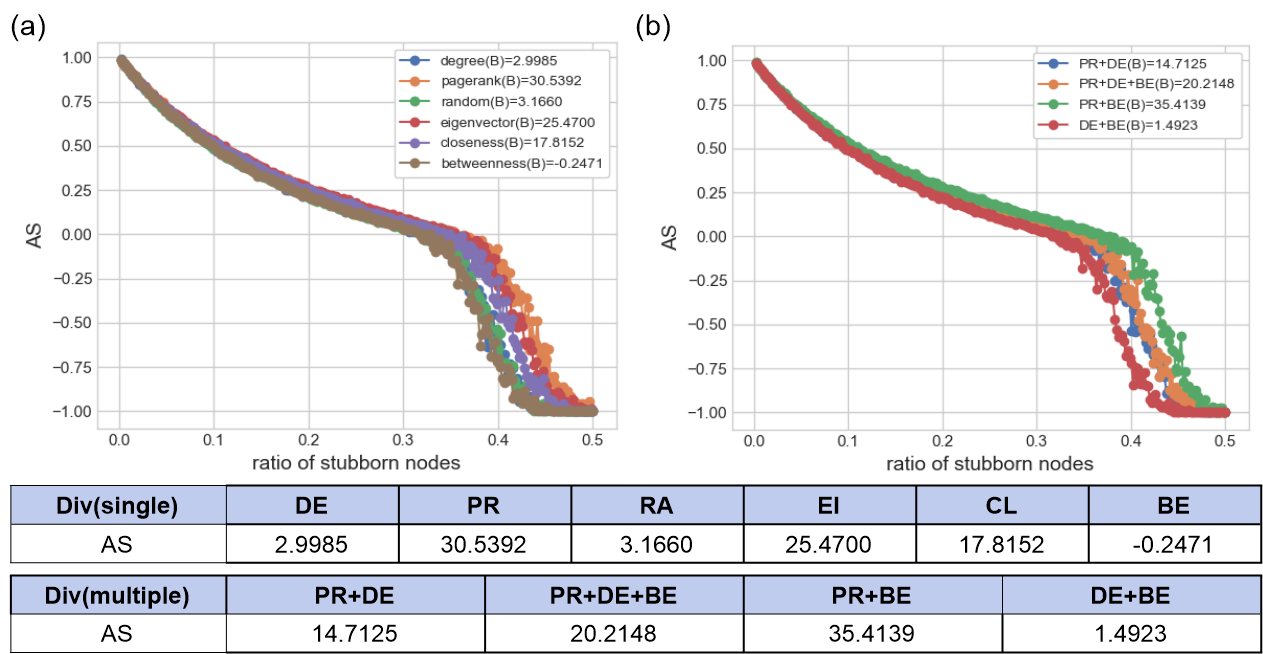
\includegraphics[width=\hsize]{figure/chap5_keynode_BA_RR_B.png}
	\caption{Key nodes on layer B in \textit{BA(3)-RR(6)} network($p=0.3, v=0.5$):
		(a) Single indicator methods, (b) Multiple indicator methods}
	\label{chap5_keynode_BA_RR_B}
\end{figure}

First, \textit{BA-RR} network would be investigated. Fig.~\ref{chap5_keynode_BA_RR_A} shows the simulation result of key nodes on layer A.\textit{PR+BE} is the most influential method. Next rank is pagerank as a single indicator. Compared with \textit{BA-BA} shown in Fig.~\ref{chap5_keynode_A}, \textit{BA-RR} has smaller \textit{AS} values and more gentle curve to change the state of network. 

Fig.~\ref{chap5_keynode_BA_RR_B} shows the simulation result of key nodes on layer B. Betweenness is the best method for finding key nodes on layer B in \textit{BA-RR} network. In this model, degree centrality is not meaningful method because degree of each node is same in \textit{RR} network. However, random and degree method is the third and fourth method for recognizing key nodes. That means other methods except for betweenness do not work for identifying key nodes. Compared with \textit{BA-BA} shown in Fig.~\ref{chap5_keynode_B}, \textit{BA-RR} has larger \textit{AS} values and more gentle curve to change the state of network. 

\begin{figure}[!htb]
	\centering
	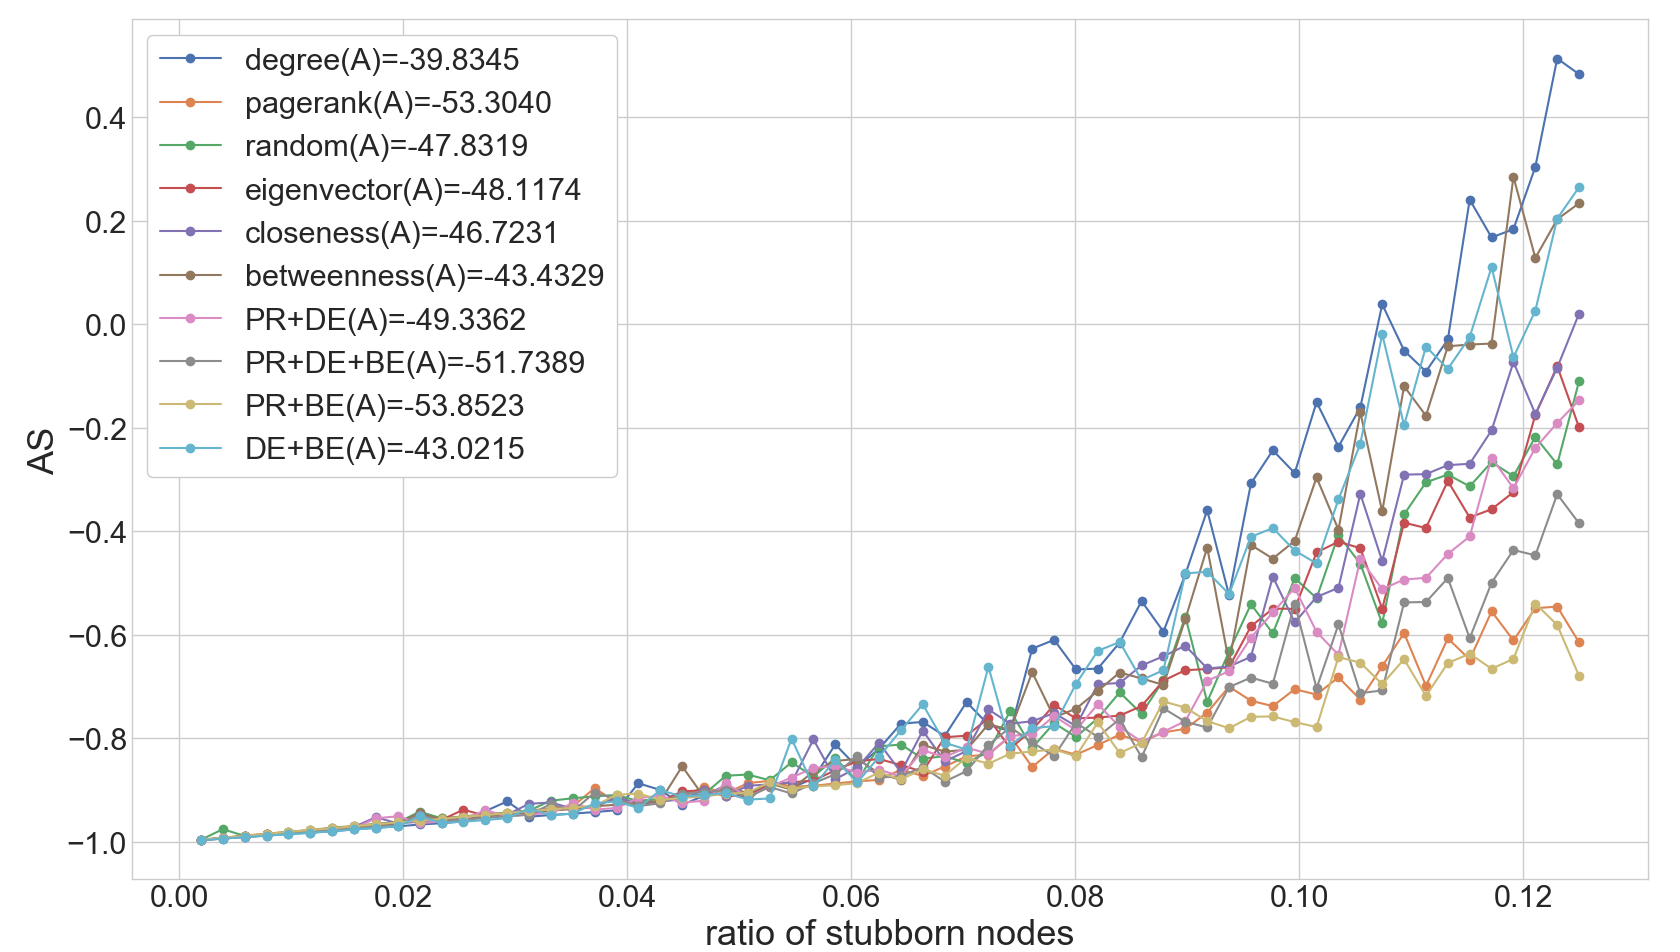
\includegraphics[width=\hsize]{figure/chap5_keynode_RR_BA_A.png}
	\caption{Key nodes on layer A in \textit{RR(6)-BA(3)} network($p=0.2, v=0.4$):
		(a) Single indicator methods, (b) Multiple indicator methods}
	\label{chap5_keynode_RR_BA_A}
\end{figure}
\begin{figure}[!htb]
	\centering
	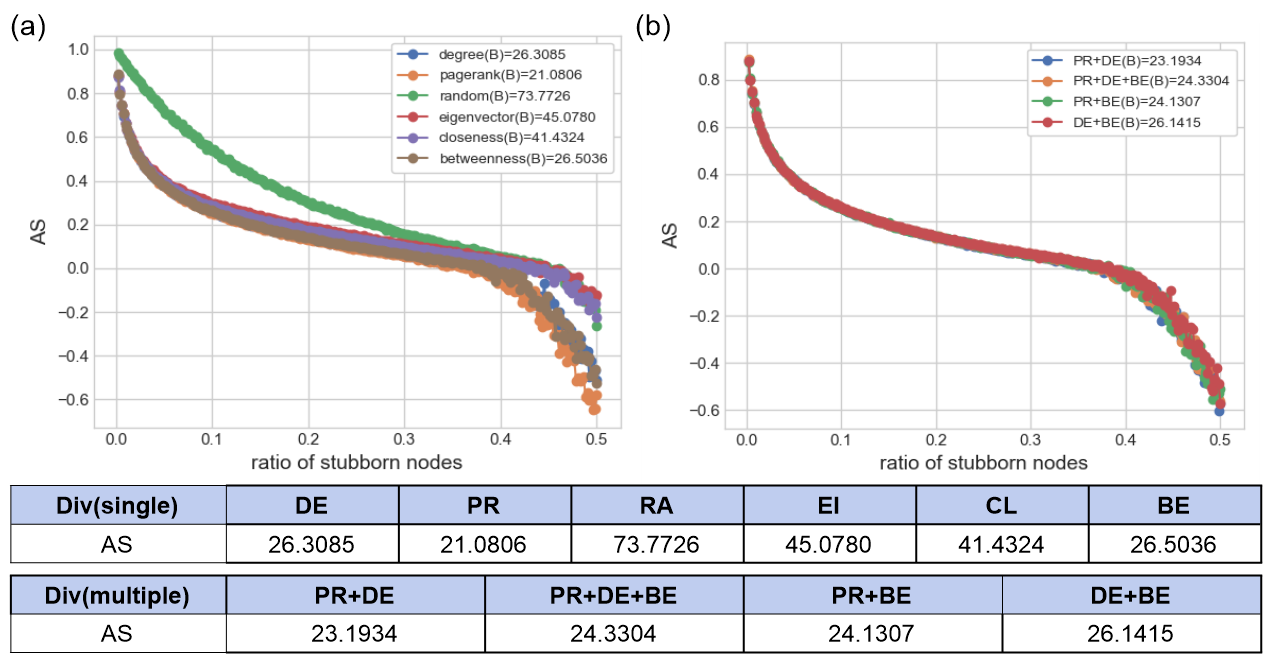
\includegraphics[width=\hsize]{figure/chap5_keynode_RR_BA_B.png}
	\caption{Key nodes on layer B in \textit{RR(6)-BA(3)} network($p=0.3, v=0.5$):
		(a) Single indicator methods, (b) Multiple indicator methods}
	\label{chap5_keynode_RR_BA_B}
\end{figure}

Next, \textit{RR-BA} network would be considered. Fig.~\ref{chap5_keynode_RR_BA_A} shows the simulation result of key nodes on layer A. The best method is degree centrality. However, in this model, degree centrality is not meaningful for recognizing key nodes because all nodes in layer A have the same degree. Here, the reason why degree centrality has good performance is analyzed as that dynamics are very efficient because nodes are sequentially changed into stubborn node and interacted(when nodes have the same node centrality, nodes are changed into stubborn nodes sequentially according to interaction order under given algorithm). And other single indicators have similar \textit{AS} values with random method. That means node centralities do not work for identifying key nodes though betweenness has better performance than other methods. Compared with \textit{BA-BA} shown in Fig.~\ref{chap5_keynode_B} , \textit{RR-BA} also has smaller \textit{AS} values and does not reach the opposite consensus yet. 

Fig.~\ref{chap5_keynode_RR_BA_B} shows the simulation result of key nodes on layer B. Pagerank has the best performance. Next rank is \textit{PR+DE}.  Compared with \textit{BA-BA} shown in Fig.~\ref{chap5_keynode_B} , \textit{RR-BA} also has larger \textit{AS} values and more gentle curve to change the state of network. 

Totally, compared with \textit{BA-BA} network, both \textit{BA-RR} and \textit{RR-BA} have more gentle curve. It could be analyzed that \textit{RR} network makes it slow for stubborn nodes to change the state of network and makes it hard to select key nodes though betweenness has good performance on \textit{RR} network.\\  

\subsection{Key nodes on two layers with different number of internal links}
Next, the case would be considered that each layer has different number of internal edges. In case that layer A has more internal links, layer A consists of \textit{BA} network with $k=4$, but layer B consists of \textit{BA} network with $k=2$. Inversely, in case that layer B has more internal links, layer B consists of \textit{BA} network with $k=4$, but layer A consists of \textit{BA} network with $k=2$. 

\begin{figure}[!htb]
	\centering
	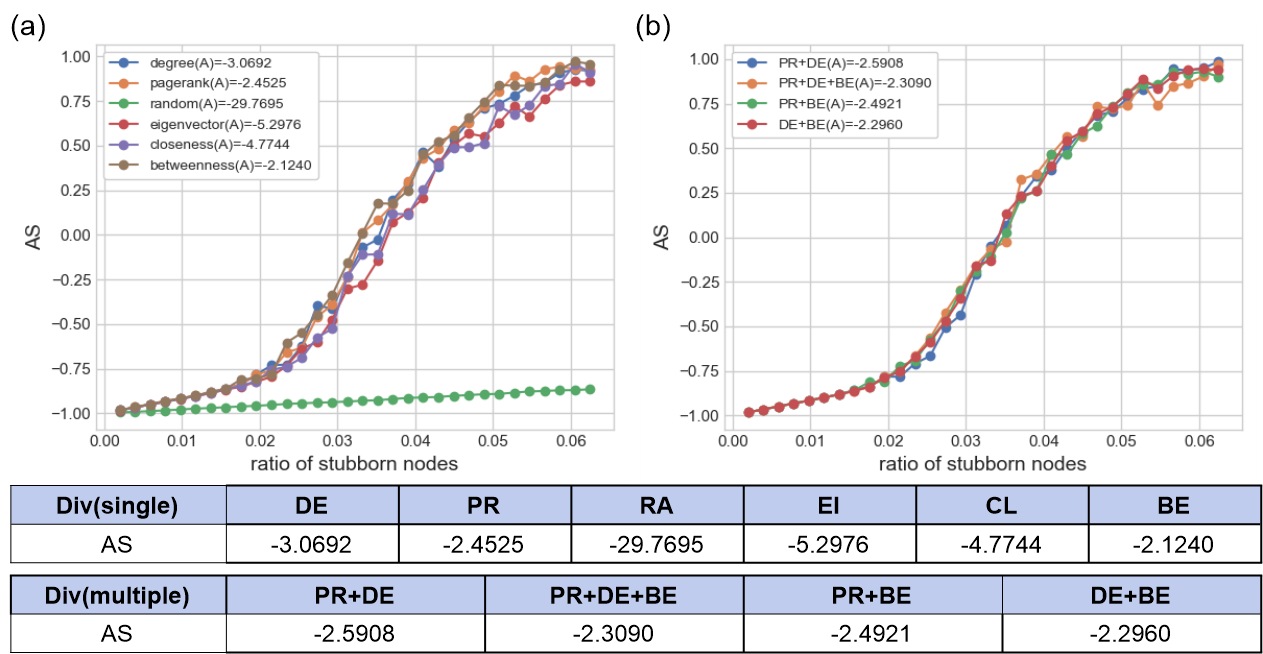
\includegraphics[width=\hsize]{figure/chap5_keynode_internal_A.png}
	\caption{Key nodes on layer A in \textit{BA(4)-BA(2)} network($p=0.15, v=0.3$):
		(a) Single indicator methods, (b) Multiple indicator methods}
	\label{chap5_keynode_internal_A}
\end{figure}
\begin{figure}[!htb]
	\centering
	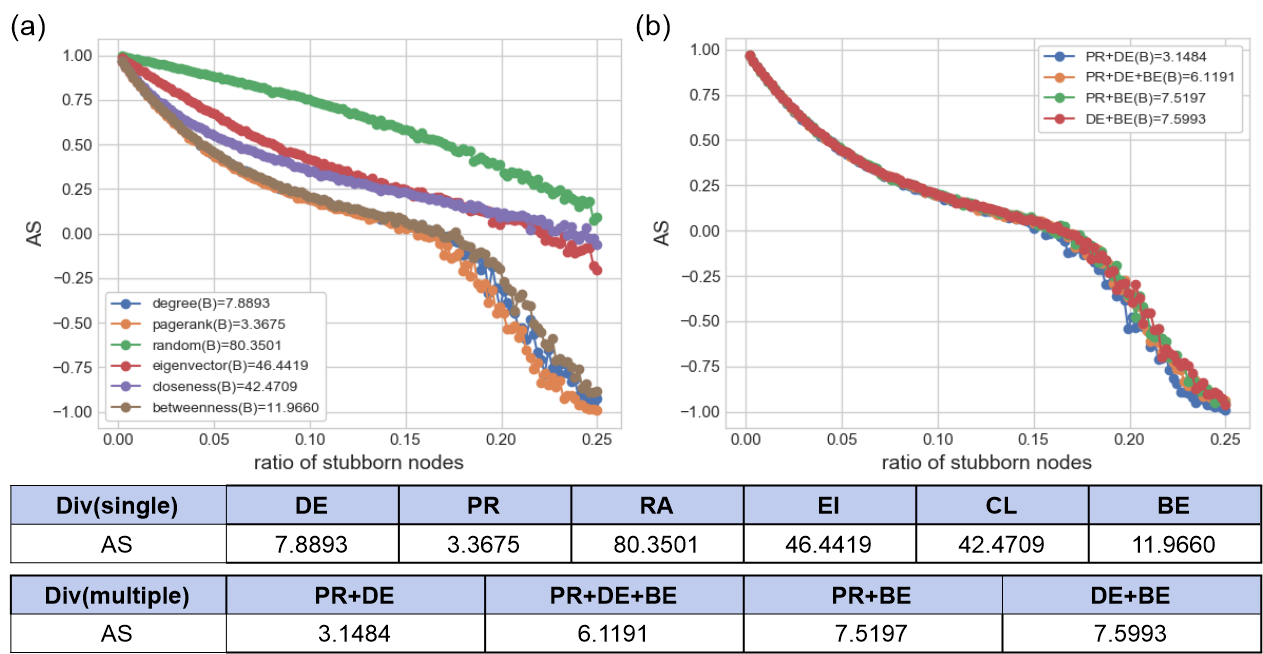
\includegraphics[width=\hsize]{figure/chap5_keynode_internal_B.png}
	\caption{Key nodes on layer B in \textit{BA(4)-BA(2)} network($p=0.2, v=0.4$):
		(a) Single indicator methods, (b) Multiple indicator methods}
	\label{chap5_keynode_internal_B}
\end{figure}

First, the case of more internal links on layer A than layer B would be investigated. 
Fig.~\ref{chap5_keynode_internal_A} shows the simulation result of key nodes on layer A in \textit{BA(4)-BA(2)} network. Betweenness has the best performance for selecting key nodes. Next ranks are \textit{DE+BE}, \textit{PR+BE} and \textit{PR+DE+BE}. Compared with the \textit{BA(2)-BA(4)} network shown in Fig.~\ref{chap5_keynode_internal_A2}, the curve of changing the state that is shown in Fig.~\ref{chap5_keynode_internal_A} is much more straight. That means consensus time is very short and it is easy to have consensus.

Fig.~\ref{chap5_keynode_internal_B} shows the simulation result of key nodes on layer B in \textit{BA(4)-BA(2)} network. \textit{PR+DE} is the most influential method. Next ranks are pagerank, \textit{PR+DE+BE} and \textit{PR+BE}. Compared with \textit{BA(2)-BA(4)} network shown in Fig.~\ref{chap5_keynode_internal_B2}, the curve of changing the state that is shown in Fig.~\ref{chap5_keynode_internal_B} is also more straight. 

Totally, compared with \textit{BA(2)-BA(4)} network, it could be analyzed that more internal edges on layer A make it easy to have consensus by stubborn nodes. 

\begin{figure}[!htb]
	\centering
	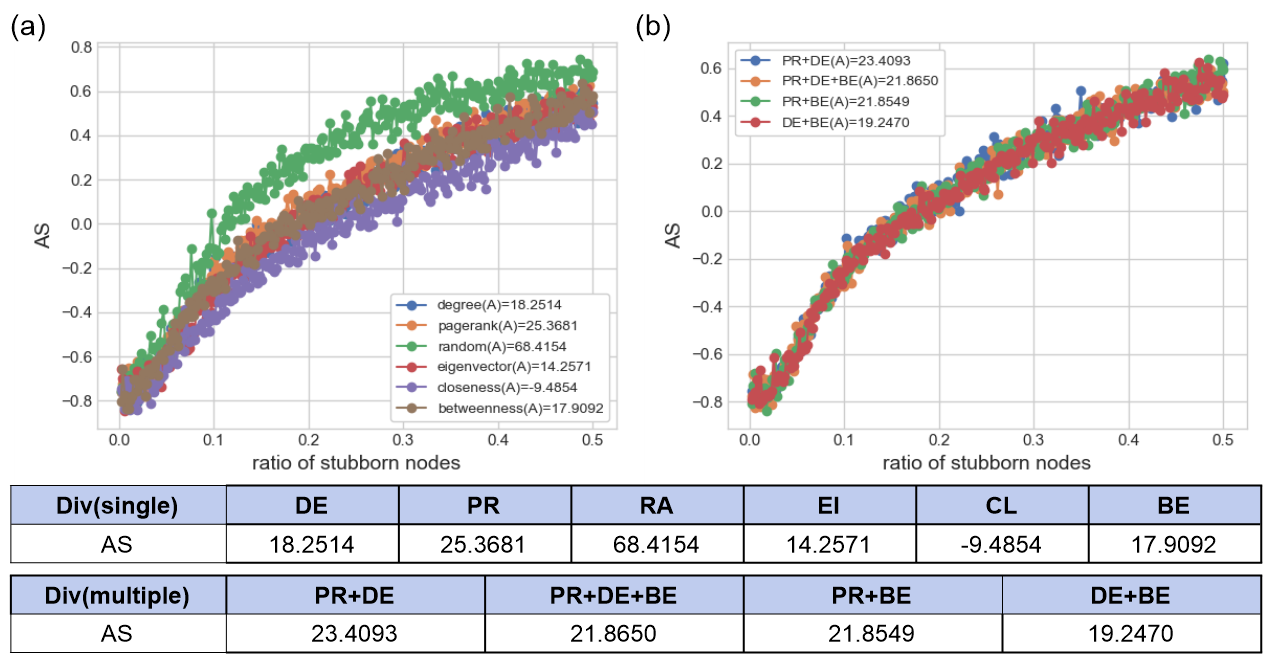
\includegraphics[width=\hsize]{figure/chap5_keynode_internal_A2.png}
	\caption{Key nodes on layer A in \textit{BA(2)-BA(4)} network($p=0.57, v=0.37$):
		(a) Single indicator methods, (b) Multiple indicator methods}
	\label{chap5_keynode_internal_A2}
\end{figure}
\begin{figure}[!htb]
	\centering
	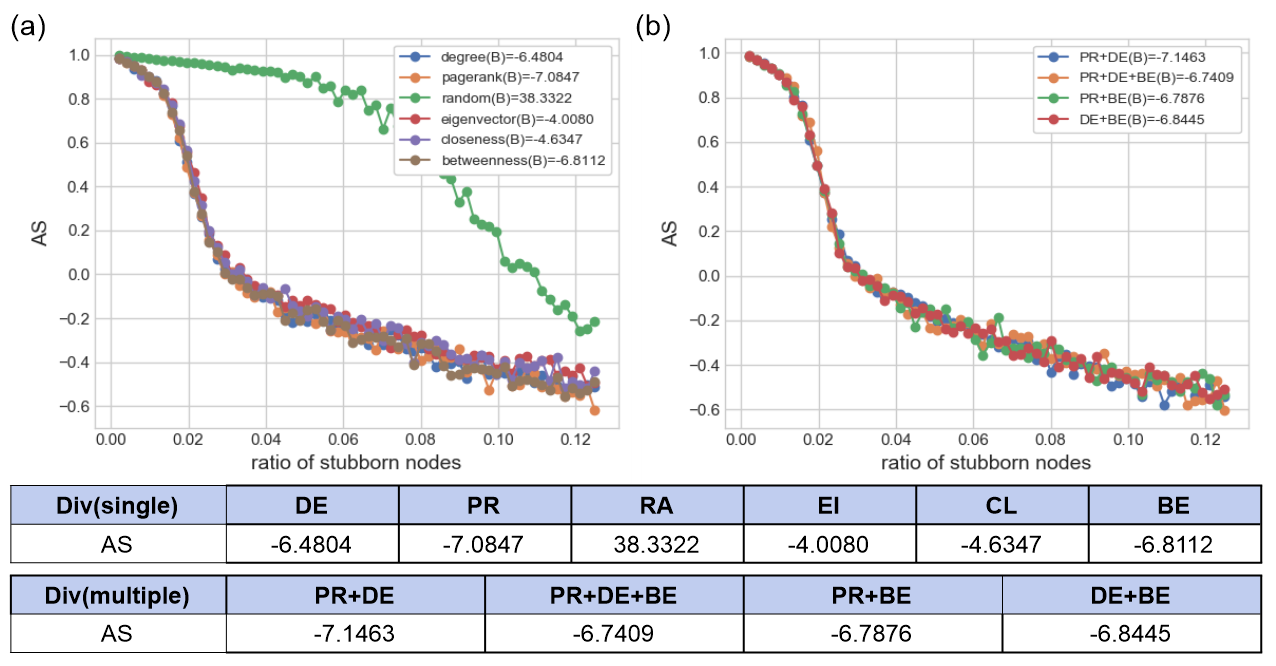
\includegraphics[width=\hsize]{figure/chap5_keynode_internal_B2.png}
	\caption{Key nodes on layer B in \textit{BA(2)-BA(4)} network($p=0.6, v=0.4$):
		(a) Single indicator methods, (b) Multiple indicator methods}
	\label{chap5_keynode_internal_B2}
\end{figure}

Next, the case of more internal links on layer B than layer A would be researched. 
Fig.~\ref{chap5_keynode_internal_A2} shows the simulation result of key nodes on layer A in \textit{BA(2)-BA(4)} network. However, the simulation results are different from other results, because random method has the best performance. That means node centralities do not work on this model. Compared with \textit{BA(4)-BA(2)} network shown in Fig.~\ref{chap5_keynode_internal_A}, the curve of changing the state that is shown in Fig.~\ref{chap5_keynode_internal_A2}  is much slower and more gentle.

Fig.~\ref{chap5_keynode_internal_B2} shows the simulation result of key nodes on layer B in \textit{BA(2)-BA(4)} network. \textit{PR+DE} has the most effective performance. Next ranks are pagerank, \textit{DE+BE} and betweenness. Compared with \textit{BA(4)-BA(2)} network shown in Fig.~\ref{chap5_keynode_internal_B}, the curve of changing the state that is shown in Fig.~\ref{chap5_keynode_internal_B2} is much faster. But consensus does not happen in this model.

Totally, compared with \textit{BA(4)-BA(2)} network, it could be analyzed that the more number of internal edges on layer B makes consensus by stubborn nodes hard. And decreasing internal edges on layer A makes it hard to select key node on layer A.\\   

\section{Conclusion}
By using node centrality and combined node centrality, key nodes on each layer have been recognized on networks of various structures. Table.~\ref{effective methods} shows total simulation results for selecting key nodes on various interconnected networks.
 
\begin{table}[!htb]
	\scriptsize
	\centering
	\caption{Effective methods for selecting key nodes on various networks}
	\label{effective methods}
	\begin{center}
		\begin{tabular}{c|c|c|c|c|c|c|c|c|c} \hline\hline
		  Div                              & A nodes & B nodes & A edges & B edges & layer & 1st method & 2nd method  & 3rd method  & remarks    \\ \hline \hline
         \multirow{1}{*}{BA(3)-BA(3)}      & 512 	 & 512     & 1,527   & 1,527   & A     & PR+BE      & PR+DE       & pagerank    &            \\ 
			                               &  	     &         &         &         & B     & pagerank   & PR+DE       & PR+BE       &		     \\ \hline   
	     \multirow{1}{*}{BA(3)-RR(6)}      & 512     & 512     & 1,527   & 1,536   & A     & PR+BE      & pagerank    & PR+DE+BE    &            \\
	                                       &         &         &         &         & B     & betweenness& DE+BE       & random      & not working\\ \hline
	     \multirow{1}{*}{RR(6)-BA(3)}      & 512     & 512     & 1,536   & 1,527   & A     & degree     & DE+BE       & betweenness & not working\\ 
	                                       &         &         &         &         & B     & pagerank   & PR+DE       & PR+BE       &            \\ \hline
		 \multirow{1}{*}{BA(4)-BA(2)}      & 512     & 512     & 2,032   & 1,020   & A     & betweenness& DE+BE       & PR+BE       &            \\ 
		                                   &         &         &         &         & B     & PR+DE      & pagerank    & PR+DE+BE    &            \\ \hline
		 \multirow{1}{*}{BA(2)-BA(4)}      & 512     & 512     & 1,020   & 2,032   & A     & random     & pagerank    & PR+DE       & not working\\ 
		                                   &         &         &         &         & B     & PR+DE      & pagerank    & DE+BE       &            \\ \hline
		 \multirow{1}{*}{HM(8) with BA(3)} & 512     & 64      & 1,527   & 183     & A     & PR+DE      & PR+BE       & pagerank    &            \\ 
		                                   &         &         &         &         & B     & random     & DE+BE       & PR+DE+BE    & not working\\ \hline
			\hline
		\end{tabular}
	\end{center}
\end{table}

Here, we could found out several facts from these simulation results. First, it could be found out that the best and most influential method is different according to network structures and layers. Second, as single indicators, pagerank, degree and betweenness are good method to select key nodes. Third, as multiple indicators, combined node centrality has good performance to recognize the key nodes on various networks. Combined node centralities are first or second effective method on all simulation models.(except not working methods)  Fourth, as the results shown in interconnected networks with different number of internal edges on each layer, the more number of links on layer A makes it easy to have consensus by stubborn nodes, and the more number of links on layer B makes it hard to make consensus by stubborn nodes. In addition, decreasing internal edges on layer A makes it hard to recognize key nodes on layer A.  Fifth, as the results shown in \textit{HM(8) with BA(3)} network, decreasing the number of nodes on layer B and increasing the number of external edges on layer B make it hard to identify key nodes on layer B and makes it easy to have consensus by stubborn nodes. Sixth, as the results shown in interconnected networks with different network types, network types have the influence to whether network can make consensus by stubborn nodes or not. Especially, it is found out that \textit{RR} network makes it slow to have consensus by stubborn nodes and makes it hard to recognize key nodes. 



